%!TEX ROOT=ctutest.tex
\chapter{Introduction}
    Personal safety in the workplace depends on the own awareness of potential threats and risks. To reduce the risk of injury or harm to health in dark situations or low-light areas, people still rely on reflective tape, a product developed in the 1970s, to keep workers safe and visible in risky situations all around the world \cite{web_article:active_lighting_systems}. 
    Tape and other reflective surfaces remain dependent on an external source of light to illuminate them. Due to this dependency, they are very limited in its overall ability to keep workers visible.
    
\section{Active Lighting Systems}
    Nowadays, proper safety measures should not only protect the person but also allow other employees to be aware of that person. The active lighting systems address this problem by helping the personnel be seen without depending on a secondary illumination source. When a person is visible from all directions, the job site is a safer place for everyone \cite{web_article:active_lighting_systems}. 
 
    SunFibre Wearable is an optic fibre lighting system from SCILIF company that emits light through optic fibres encased in a textile coating. Side-emitting optic fibres provide visibility in all directions up to a distance of 3 kilometres. The properties of the textile coated optic fibres allow easy sewing into products such as jackets or vests, guarantee mechanical durability and washability and do not produce any heat.
    
    \begin{figure} [!ht]
        \centering
        \caption{SunFibre Wearable active lighting system}

        \begin{subfigure}[b]{0.495\textwidth}
            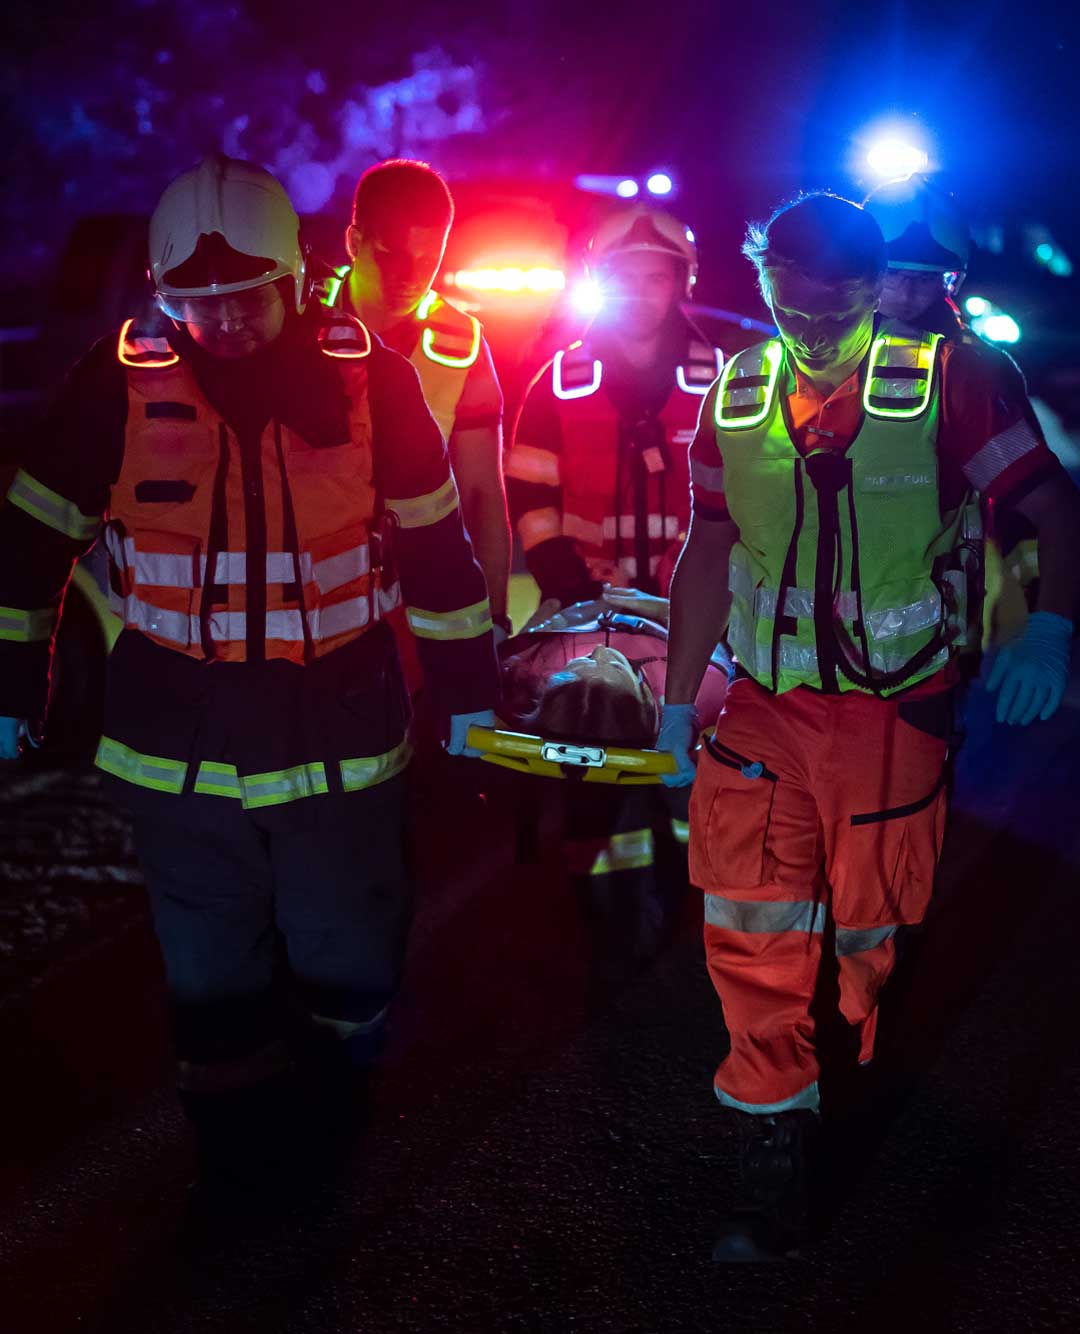
\includegraphics[width=\textwidth]{01.INTRO/Figs/active_lighting_system01.jpg}
        \end{subfigure}
         \hfill
        \begin{subfigure}[b]{0.496\textwidth}
             \centering
             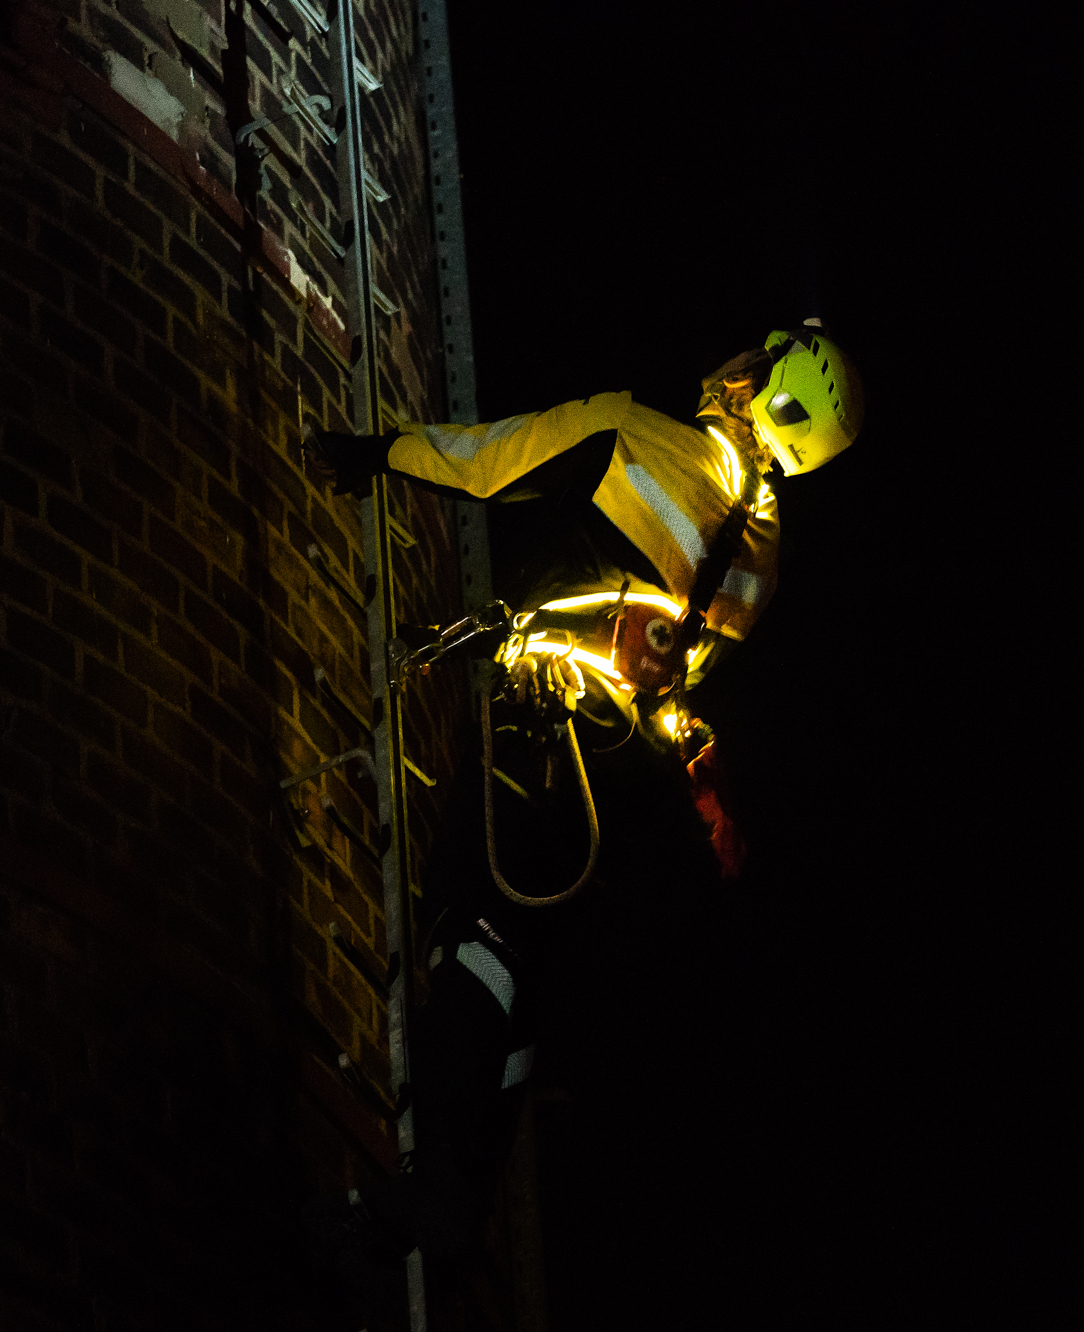
\includegraphics[width=\textwidth]{01.INTRO/Figs/active_lighting_system03.jpg}
         \end{subfigure}
    \end{figure}      
     
    
\section{Remote Control of Active Lighting Systems}
    \todo{TO BE DONE ...}

\section{Motivation}
    This thesis aims at designing and implementing a solution for remote control of SCILIF active lighting system. The objective is to develop a functional prototype allowing local and BLE-based remote control as well as advanced features such as gesture control and RFID control. Because the hardware design was done externally, the main tasks are firmware and mobile application development.
    
     
    \begin{titleitemize}{A List of Tasks:}
        \item Firmware implementation of control units allowing local and remote control
        \item Implementation of mechanisms for firmware updates
        \item Implementation of monitoring and control applications for current mainstream mobile platforms
        \item Implementation of advanced features such as gesture control and  RFID based control etc.
        \item Documentation of projects and source code repositories for future development and preparation of manuals and scripts for devices bring-up in planned serial production
    \end{titleitemize}
 


    
    
  